\documentclass[12pt]{book}

\usepackage{suthesis-2e}
\usepackage{url}
\usepackage{graphicx}
\usepackage{caption}
\usepackage{subcaption}
\usepackage[inline]{enumitem}
\usepackage{eso-pic}
\usepackage{float}

\counterwithout{figure}{chapter}
\counterwithout{table}{chapter}


\begin{document}

    \title{Comparing Conditional Random Fields and Long-Short-Term-Memory Networks for Named Entity Recognition}
    \author{Josef Gugglberger}
    \principaladviser{Dipl.-Ing.Clemens Sauerwein, PhD}
	\AddToShipoutPicture*{
		\put(-55,55){
			\parbox[b]{\paperwidth}{
				\hfill \includegraphics[scale=0.35]{img/uni-watermark}
			}
		}
	}
    \beforepreface
    \prefacesection{Abstract} 
    
    Named entity recognition (NER) is one of the most addressed problems in research in the field of natural language processing (NLP). Many conferences and workshops, including CoNLL 2002-2003 and W-NUT 2015-2019 among others, launched shared tasks focusing on NER or similar NLP tasks. Traditional NER systems usually require a lot of manual feature engineering to train the system to an acceptable performance. Nowadays, most state-of-the-art natural language processing systems are using deep learning algorithms for NER. 
    
    Aim of this thesis is to conduct a practical study, comparing two different approaches of NER systems regarding their performance on different datasets. Furthermore, this thesis investigates, if the traditional machine learning techniques can compete with modern deep learning techniques, and if there is still a need for them in NER systems. For this reason, two NER systems were implemented and compared to each other. While one system was implemented with a traditional machine learning approach (Conditional Random Fields), the second system was realised with a deep learning approach (Long-Short-Term-Memory networks).
    
    The systems were evaluated on two different datasets, the CoNLL 2003 and the W-NUT 2017 dataset, based on the metrics precision, recall and F1-score.
    It was shown that the deep learning approach outperforms the machine learning approach on the CoNLL 2003 dataset. However, on the noisy W-NUT 2017 dataset, the machine learning approach performed slightly better.

 	\afterpreface
 	
 	
    \chapter{Introduction}
    
    Named Entity Recognition (NER) is a well-studied process in natural language processing (NLP). It aims to locate and classify named entities in unstructured text.
    
    With the rise of deep learning from 2015 onwards, the methods to perform NER have changed in research. The traditional machine learning approaches like Hidden Markov Models and Conditional Random Fields (CRF) were mostly replaced by a special type of Recurrent Neural Networks, so-called Long-Short-Term-Memory (LSTM) neural networks. 
    
    The first approach to apply LSTM networks for Named Entity Recognition was done already in the year 2003, in the paper \cite{hammerton-2003-named}. Hammerton et al. proposed an LSTM based approach, that utilised a so called SARDNET \cite{james1995sardnet} for representing words. However, due to the lack of computational power back then, and the limited quality of the word representations provided by SARDNET, the performance was far behind state-of-the-art methods.
    In 2015, Huang et al. \cite{huang2015bidirectional} showed various LSTM networks that reached state-of-the-art performance. Also, the currently best performing NER system on the CoNLL 2003 \cite{tjongkimsang2003conll} dataset, called \textit{Flair} \cite{akbik2018contextual}, makes use of an LSTM network. \\
    
    The question of interest in this thesis is: Are there datasets, on which a traditional machine learning approach performs better than a modern deep learning approach, and if so, what kind of datasets are those?
    
    To answer this question, a case study was performed. This thesis compares the performance of one specific instance of a machine learning approach, and one specific instance of a deep learning approach on two well-studied datasets. The study was conducted by implementing two NER systems: the first system is based on CRFs, while the second system implements two variations of an LSTM network: the first variant implements a bidirectional LSTM (BI-LSTM) network, and the second one a BI-LSTM-CRF network, which is a BI-LSTM network with an additional CRF layer added before the output. The performance of the tools are compared in terms of precision, recall and F1-score on the CoNLL 2003 and the W-NUT 2017 \cite{derczynski2017results} dataset. The nature of the two datasets is very different. On the other hand, the CoNLL 2003 dataset provides clean texts from newswire articles, while on the other hand, the W-NUT dataset contains texts that are noisy and user-generated (e.g. social media posts).\\
    
    The remainder of this thesis is structured as follows: Chapter \ref{chap:backround} is about related work and some background information on Named Entity Recognition, CRFs and LSTM networks. Chapter \ref{chap:method} describes the details of the two implementations of the NER system. Chapter \ref{chap:evaluation} compares, evaluates and discusses the results generated by the implemented NER systems. Finally, Chapter \ref{chap:conclusion} concludes and gives an outlook on what could be done in the future.
   
	\chapter{Background \& Related Work}
	\label{chap:backround}
	
	This chapter presents basic background information of the topics NER (Section \ref{sec:ner}), CRFs (Section \ref{sec:crf}) and LSTM networks (Section \ref{sec:lstm}). The last section, Section \ref{sec:relatedwork}, summarizes recent work.

	
	\section{Named Entity Recognition}
	\label{sec:ner}
	
	\textit{Named Entity Recognition} is the task of locating and classifying named entities in unstructured text. A named entity is classified into a predefined set of categories, which can be names of people, locations, companies, etc. A named entity describes something physical (person, location, etc.). For example: \\
	
	[James :PER] visited the [Eiffel :LOC] [Tower :LOC] in [2012 :TIME]. \\
	
	This sentence contains three named entities. \textit{James} is a person name, \textit{Eiffel Tower} is a location, and \textit{2012} is a time expression. Words that do not represent named entities are labelled with a special category, that represents that the word is no named entity. The notation of this special category is usually 'O'. Examples often omit this category, which means that every word that was not labelled, is in that category. \\

	
	Named Entity Recognition is a so called sequence labelling task, because every input (word) appears in a sequence (sentence), and every input has to be labelled.
	 
	A \textit{mention} is a phrase in the text that refers to that entity with a name \cite{MAL-013}. For example, the terms \textit{U.S.A} and \textit{the United States of America} are two different phrases that refer to the same named entity.
	The categories in which the named entities are classified depends strongly on the domain where the NER system will be deployed, but the categories \textit{person}, \textit{location}, \textit{organization} and \textit{miscellaneous} are often used in research, for example in \cite{tjongkimsang2003conll}.

	
	\section{Conditional Random Fields}
	\label{sec:crf}
	
	The NER system based on the machine learning approach was implemented with an algorithm that uses Conditional Random Fields (CRF).
	A \textit{Conditional Random Field}, initially proposed in \cite{lafferty2001conditional}, is a discriminative probabilistic classifier. In contrast to a discrete classifier (like the naive Bayes classifier), it makes its prediction not just based on the input sample, but also based on the context of the input sample. For that reason, CRFs are very suitable for sequence labelling tasks. This is also an important ability in the domain of natural language processing, especially in part-of-speech tagging and Named Entity Recognition. 
	
	To model the context of a sample we have to define feature functions, which have to be defined in a way that expresses some characteristic that is present in the training data and that is expected to be present in the test data. A feature function has to form:
	
	\begin{equation}
	f(y_t, y_{t-1}, x_t)
	\end{equation}
	
	where $y_t$ is the current label, $y_{t-1}$ is the previous label and $x_t$ are the samples from the input sequence that the feature function needs to calculate the feature. The Conditional Random Field, as defined in \cite{MAL-013}, is then:
	
	\begin{equation}
	p(y|x) = \frac{1}{Z(x)} \prod_{t=1}^T exp(\sum_{k=1}^{K} \theta_k f_k(y_t, y_{t-1}, x_t))
	\end{equation}
	
	where $Z(x)$ is an normalization function:
	
	\begin{equation}
	Z(x) = \sum_{y} \prod_{t=1}^{T} exp(\sum_{k=1}^{K} \theta_k f_k(y_t, y_{t-1}, x_t))
	\end{equation}
	
	and $\theta$ is a parameter vector. The values of the parameter vector $\theta$ have to be learned from the training data, usually via Maximum Likelihood Estimation. Each feature function is multiplied by its parameter vector and then summed up. To take the context into account, this is computed for every time-step, which are then multiplied by each other. The result is $p(y|x)$, which is the probability of $y$ (the named entity label) over $x$ (the word). This probability is calculated for each named entity category, and the maximum is chosen as the prediction.
	
	\section{LSTM Networks}
	\label{sec:lstm}
	
	The NER system based on a deep learning approach was implemented with Long-Short-Term-Memory (LSTM) neural networks.
	An LSTM network is a special type of Recurrent Neural Network (RNN). In contrast to a feed-forward neural network, like for example a Convolutional Neural Network, where the data flows only in one direction (from input to output), the data can flow in cycles in a RNN. This property makes a RNN able to memorize inputs, which causes them to be suitable for sequence labelling tasks.
	RNNs have been considered difficult to train a long time, especially when they are trained to recognise long-term dependencies. The problems that arise in such cases is called the \textit{vanishing} and \textit{exploding} gradient problem \cite{lipton2015critical}. The vanishing gradient problem occurs because the gradients of back-propagation are multiplied by each other to get the dependencies from the previous steps. This problem makes RNNs almost unusable for many NLP tasks because natural language can rely heavily on long-term dependencies.
	
	LSTM networks, proposed in \cite{hochreiter1997long}, were designed to overcome the issue that RNNs have with long-term dependencies. Each LSTM cell holds an internal memory state, which is added (instead of multiplied) to the process input. The time dependence in the cell is determined by the forget gate.
	
	Figure \ref{img:lstm} shows an LSTM cell, as it is described in \cite{huang2015bidirectional}. The data flows from left to right. $x$ is the sequence sample at the current time step, $o_{-1}$ is the output of the previous LSTM cell. The input $x$ and $o_{-1}$ are concatenated at the first step and is squashed between -1 and 1 by a $tanh$ function afterwards. This can be expressed by the formula:
	
	\begin{equation}
		g = tanh(b^g + x U^g + o_{-1} V^g)
		\label{eq:input}
	\end{equation}
	
	where $b^g$ is the input bias, $U^g$ and $V^g$ are weights from the input and the previous LSTM cell.
	
	The result of formula \ref{eq:input}, $g$, is then multiplied element-wise with the output of the input gate. The input gate is a sigmoid function, mapping inputs between 0 and 1, this can turn on and off parts of the input. The mathematical expression of the input gate is:
	
	\begin{equation}
		i = \sigma (b^i + x U^i + o_{-1} V^i)
		\label{eq:inputgate}
	\end{equation}
	
	where $b^i$ is the input gate bias, $U^i$ and $V^i$ are weights from the input gate and the previous LSTM cell.
	
	The next stage in the cell is called the forget gate. The new variable $s$ represents the internal state of the LSTM cell. The internal state is delayed by one step (represented by $s_{-1}$) and added to the output of the input gate. A sigmoid function determines which words can be forgotten (close to 0), and which words need to be remembered (output close to 1). This can be expressed by the formula:
	
	\begin{equation}
		f = \sigma (b^f + x U^f + o_{-1} V^f)
		\label{eq:forgetgate}
	\end{equation}
	
	where $b^f$ is the forget gate bias, $U^f$ and $V^f$ are weights from the forget gate and the previous LSTM cell. 
	The output of the forget gate stage, $s$ is expressed by:
	
	\begin{equation}
		s = s_{-1} \cdot f + g \cdot i
	\end{equation}
	
	
	The last stage is the output gate, which operates in the same way as the input gate. The output is squashed between -1 and 1 by a hyperbolic tangent function and the output gate with a sigmoid function determines which values to output. The output gate can be defined as:
	
	\begin{equation}
		h = \sigma (b^h + x U^h + h_{-1} V^h)
		\label{eq:outgate}
	\end{equation}
	
	where $b^h$ is the output gate bias, $U^h$ and $V^h$ are weights from the output gate and the previous LSTM cell. 
	Finally, the output of the LSTM cell can be written down as:
	
	\begin{equation}
		o = tanh(s) \cdot h
		\label{eq:out}
	\end{equation}
	
	\begin{figure}
		\begin{center}
			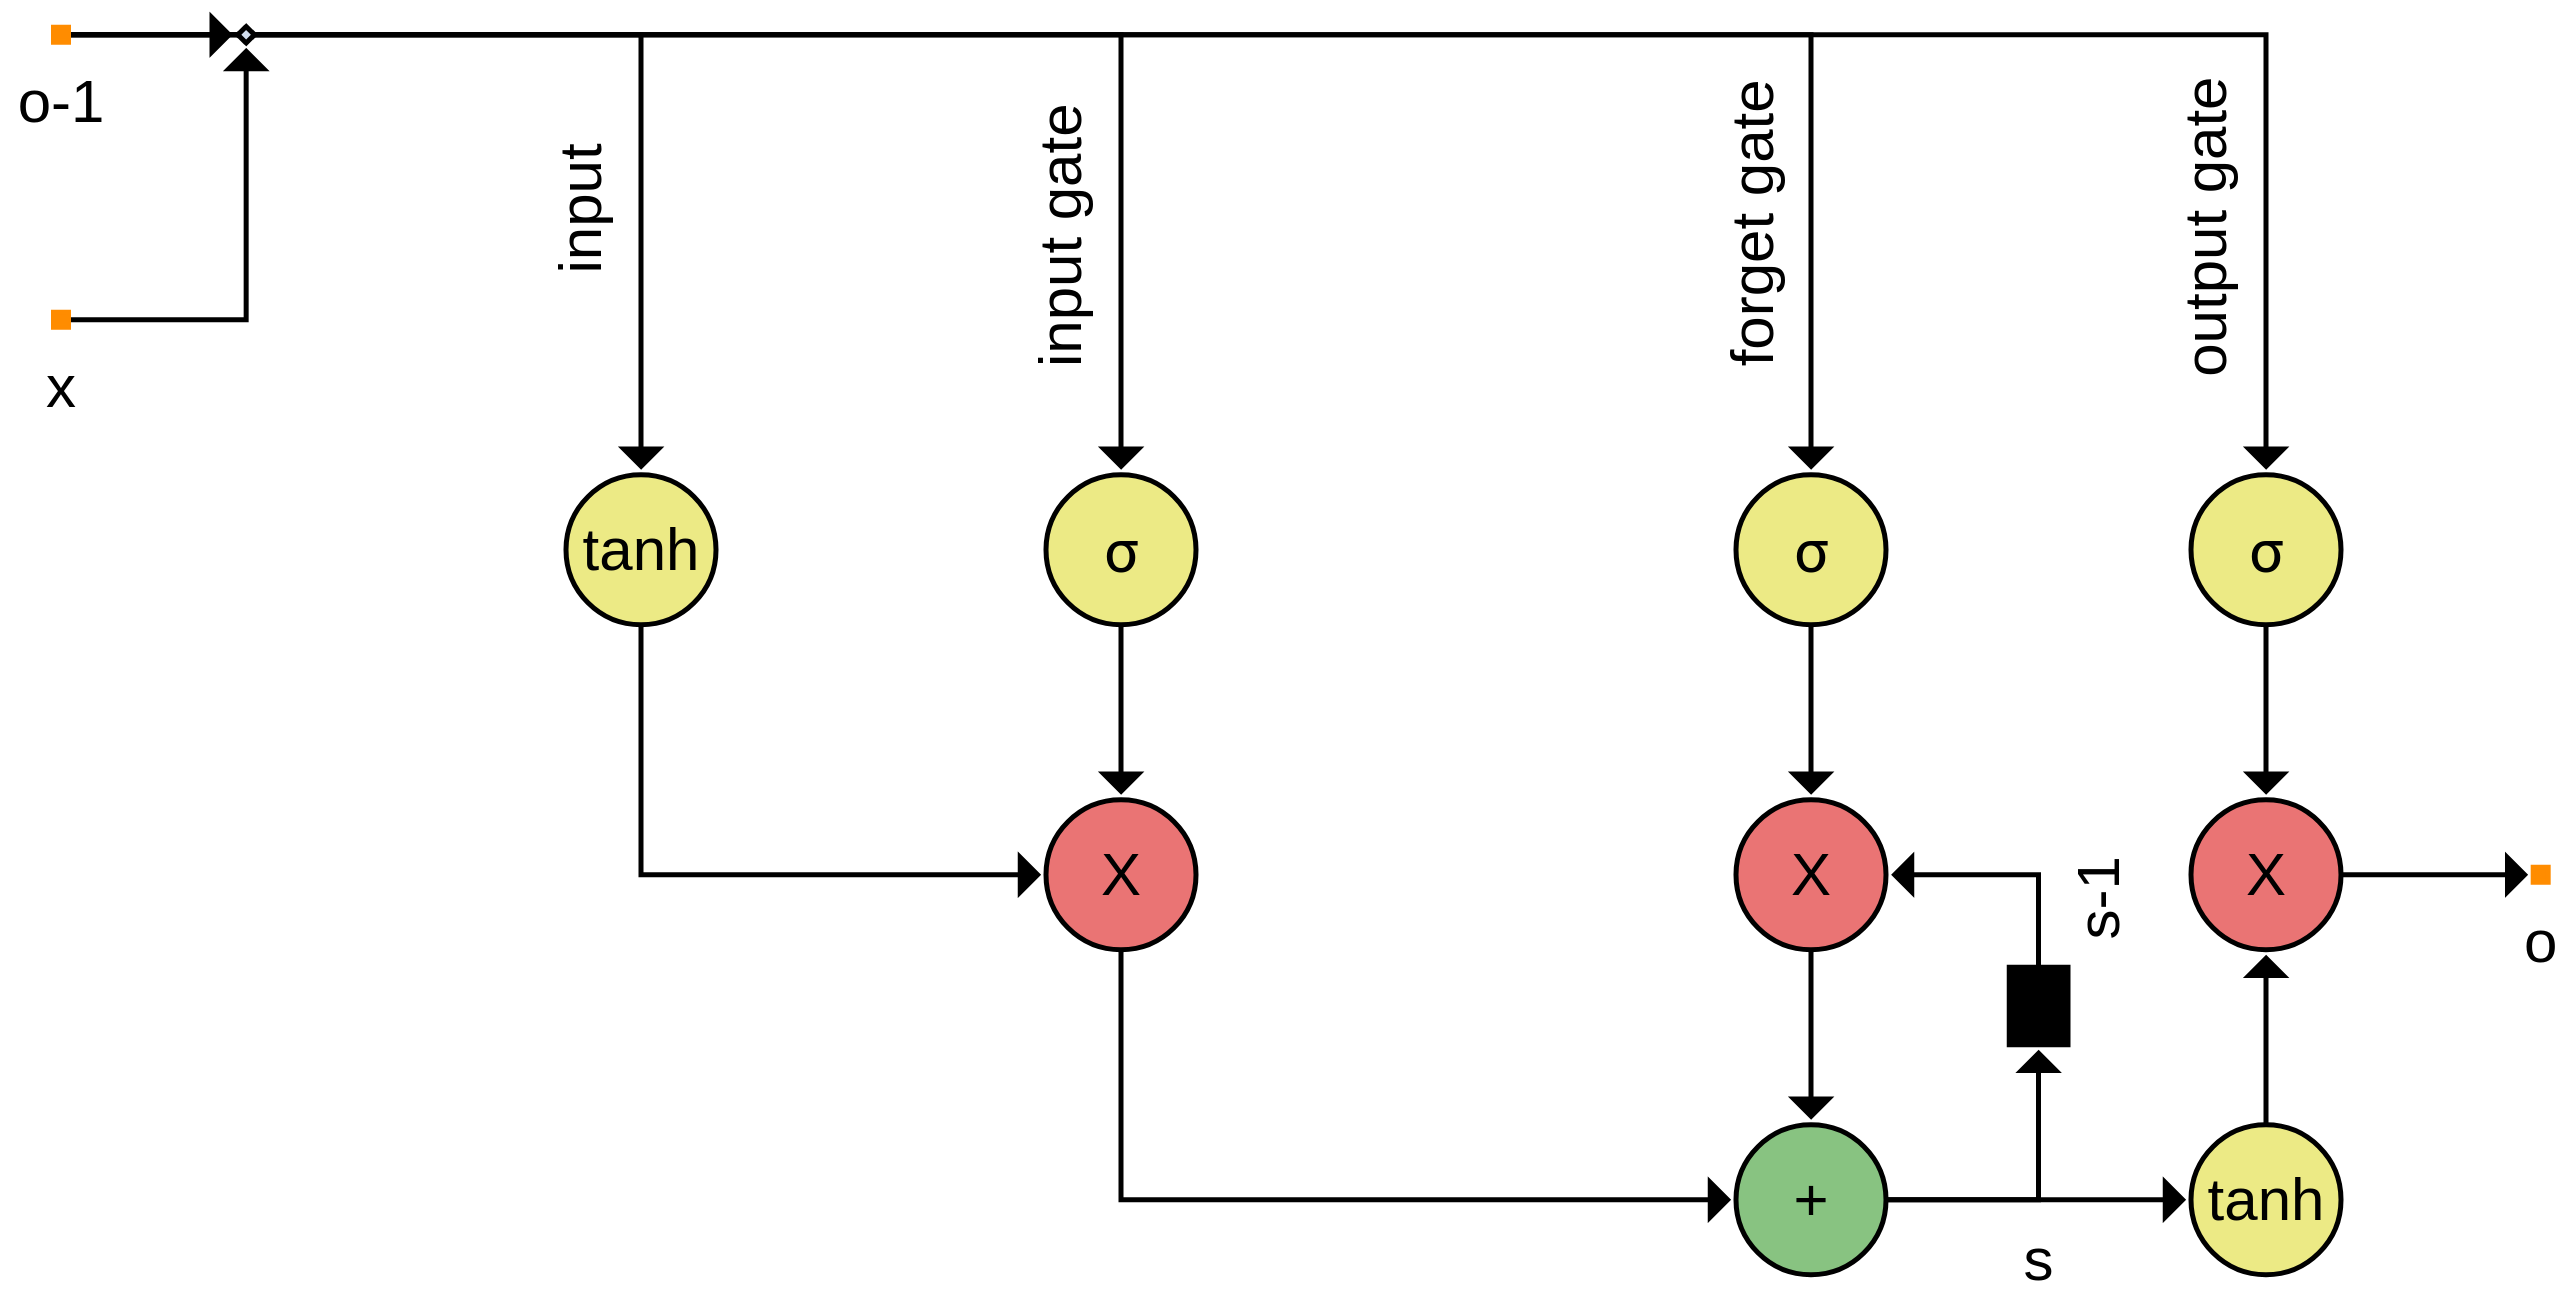
\includegraphics[width=0.75\linewidth]{img/lstm.png}
		\end{center}
		\caption{Overview of an LSTM cell. Yellow nodes represent a hidden layer, red and green nodes represent a element-wise operation \cite{lstmtut}.}	
		\label{img:lstm}
	\end{figure}
	
	\section{Related Work}
	\label{sec:relatedwork}
	
	A comparison between CRF and LSTM networks was already proposed by Nikola Ljube{\v{s}}i{\'c} in \cite{ljubevsic2018comparing}. However, there are some differences in the scope of the study: first, the analysis that was made there focuses on Slovene, Croatian and Serbian data, second, the paper concentrated on morphosyntactic tagging instead of NER, and third, the study was just based on short and noisy posts from Twitter. The author concluded that both approaches performed with good and also similar results. He conducted a error-analysis, which showed that the neural network worked better at long-range dependencies, while CRFs performed slightly better at local dependencies. Furthermore, the author claims that the neural network performed better in comparison to the CRF system with increasing \textit{non-standardness} of the text.
	
	Tjong Kim Sang et al. compared a wide range of NER systems in the CoNLL 2002 \cite{sangerik} and CoNLL 2003 \cite{tjongkimsang2003conll} shared tasks. The CoNLL 2002 task focused on NER for Dutch and Spanish texts, while the CoNLL 2003 task provided datasets for English and German. 
	In \cite{tjongkimsang2003conll}, the performances of 16 teams were evaluated and compared. Back then, deep learning algorithms were not capable of achieving good results in NER. Therefore, machine learning algorithms dominated the shared task. The three best performing NER systems used Maximum Entropy Models, and four systems used Hidden Markov Models. Conditional Random Fields were used by one team, which achieved the 9th place in the competition.
	
	Another shared task, which was launched as the workshop for noisy user-generated text (W-NUT) for the 5th time in 2019, focuses on NER and similar NLP tasks on noisy texts.
	In the W-NUT 2017 \cite{derczynski2017results} shared tasked, Aguilar et al. achieved the best results of the competition with the approach proposed in \cite{aguilar2019multi}. The authors came up with a multi-task neural network. A Convolutional Neural Network was used to capture orthographic features on the character level. A bidirectional LSTM network was used for contextual and syntactic features. Gazetteers were deployed to cover well-known entities. The output of the trained network is then passed to a CRF classifier, to make use of its good sequence labelling abilities. Also the second and third ranked NER systems, published by Von D{\"a}niken et al. and Lin et al. in \cite{von2017transfer} and \cite{lin2017multi}, used a combination of a bidirectional LSTM network and a CRF classifier.
	
	\chapter{Research Method}
	\label{chap:method}
	
	Aim of this work was to conduct a practical study comparing a CRF approach and an LSTM approach for NER. Two NER systems were developed, trained and tested by two different datasets. This chapter provides the implementation details of both approaches.
	
	Figure \ref{fig:overview} shows a high-level overview of the training and testing phase of a Named Entity Recognition system. The upper half of the figure shows the training process, which starts with an annotated document taken from the dataset. The dataset is then parsed and split up into the document itself and the corresponding labels. The document is usually one sentence, while the labels are a sequence of the predefined named entity categories. In the next step, features are extracted from the document. The last step in the training process is to pass the features with the corresponding label into the machine learning algorithm. The output of this phase is a file, which represents the machine learning model. 
	The lower half of the figure shows the testing phase. It starts in the same way as the train-phase, by splitting up the annotated document into the document and the labels of the document. After feature extraction, the features are passed together with the model file, which was generated in the test phase, into the prediction function. The output of the prediction is a file that assigns each word in a document to a label. 
	The output of the prediction and the original labels are passed into the evaluation function. There the predicted labels are compared with the original ones, and metrics like precision, recall and F1-score are computed and outputted.
	The process of training and testing is done in the same way in both implementations. The differences lie in the way the features are extracted, and how the system is trained and predicting.
	
	\begin{figure}
		\begin{center}
			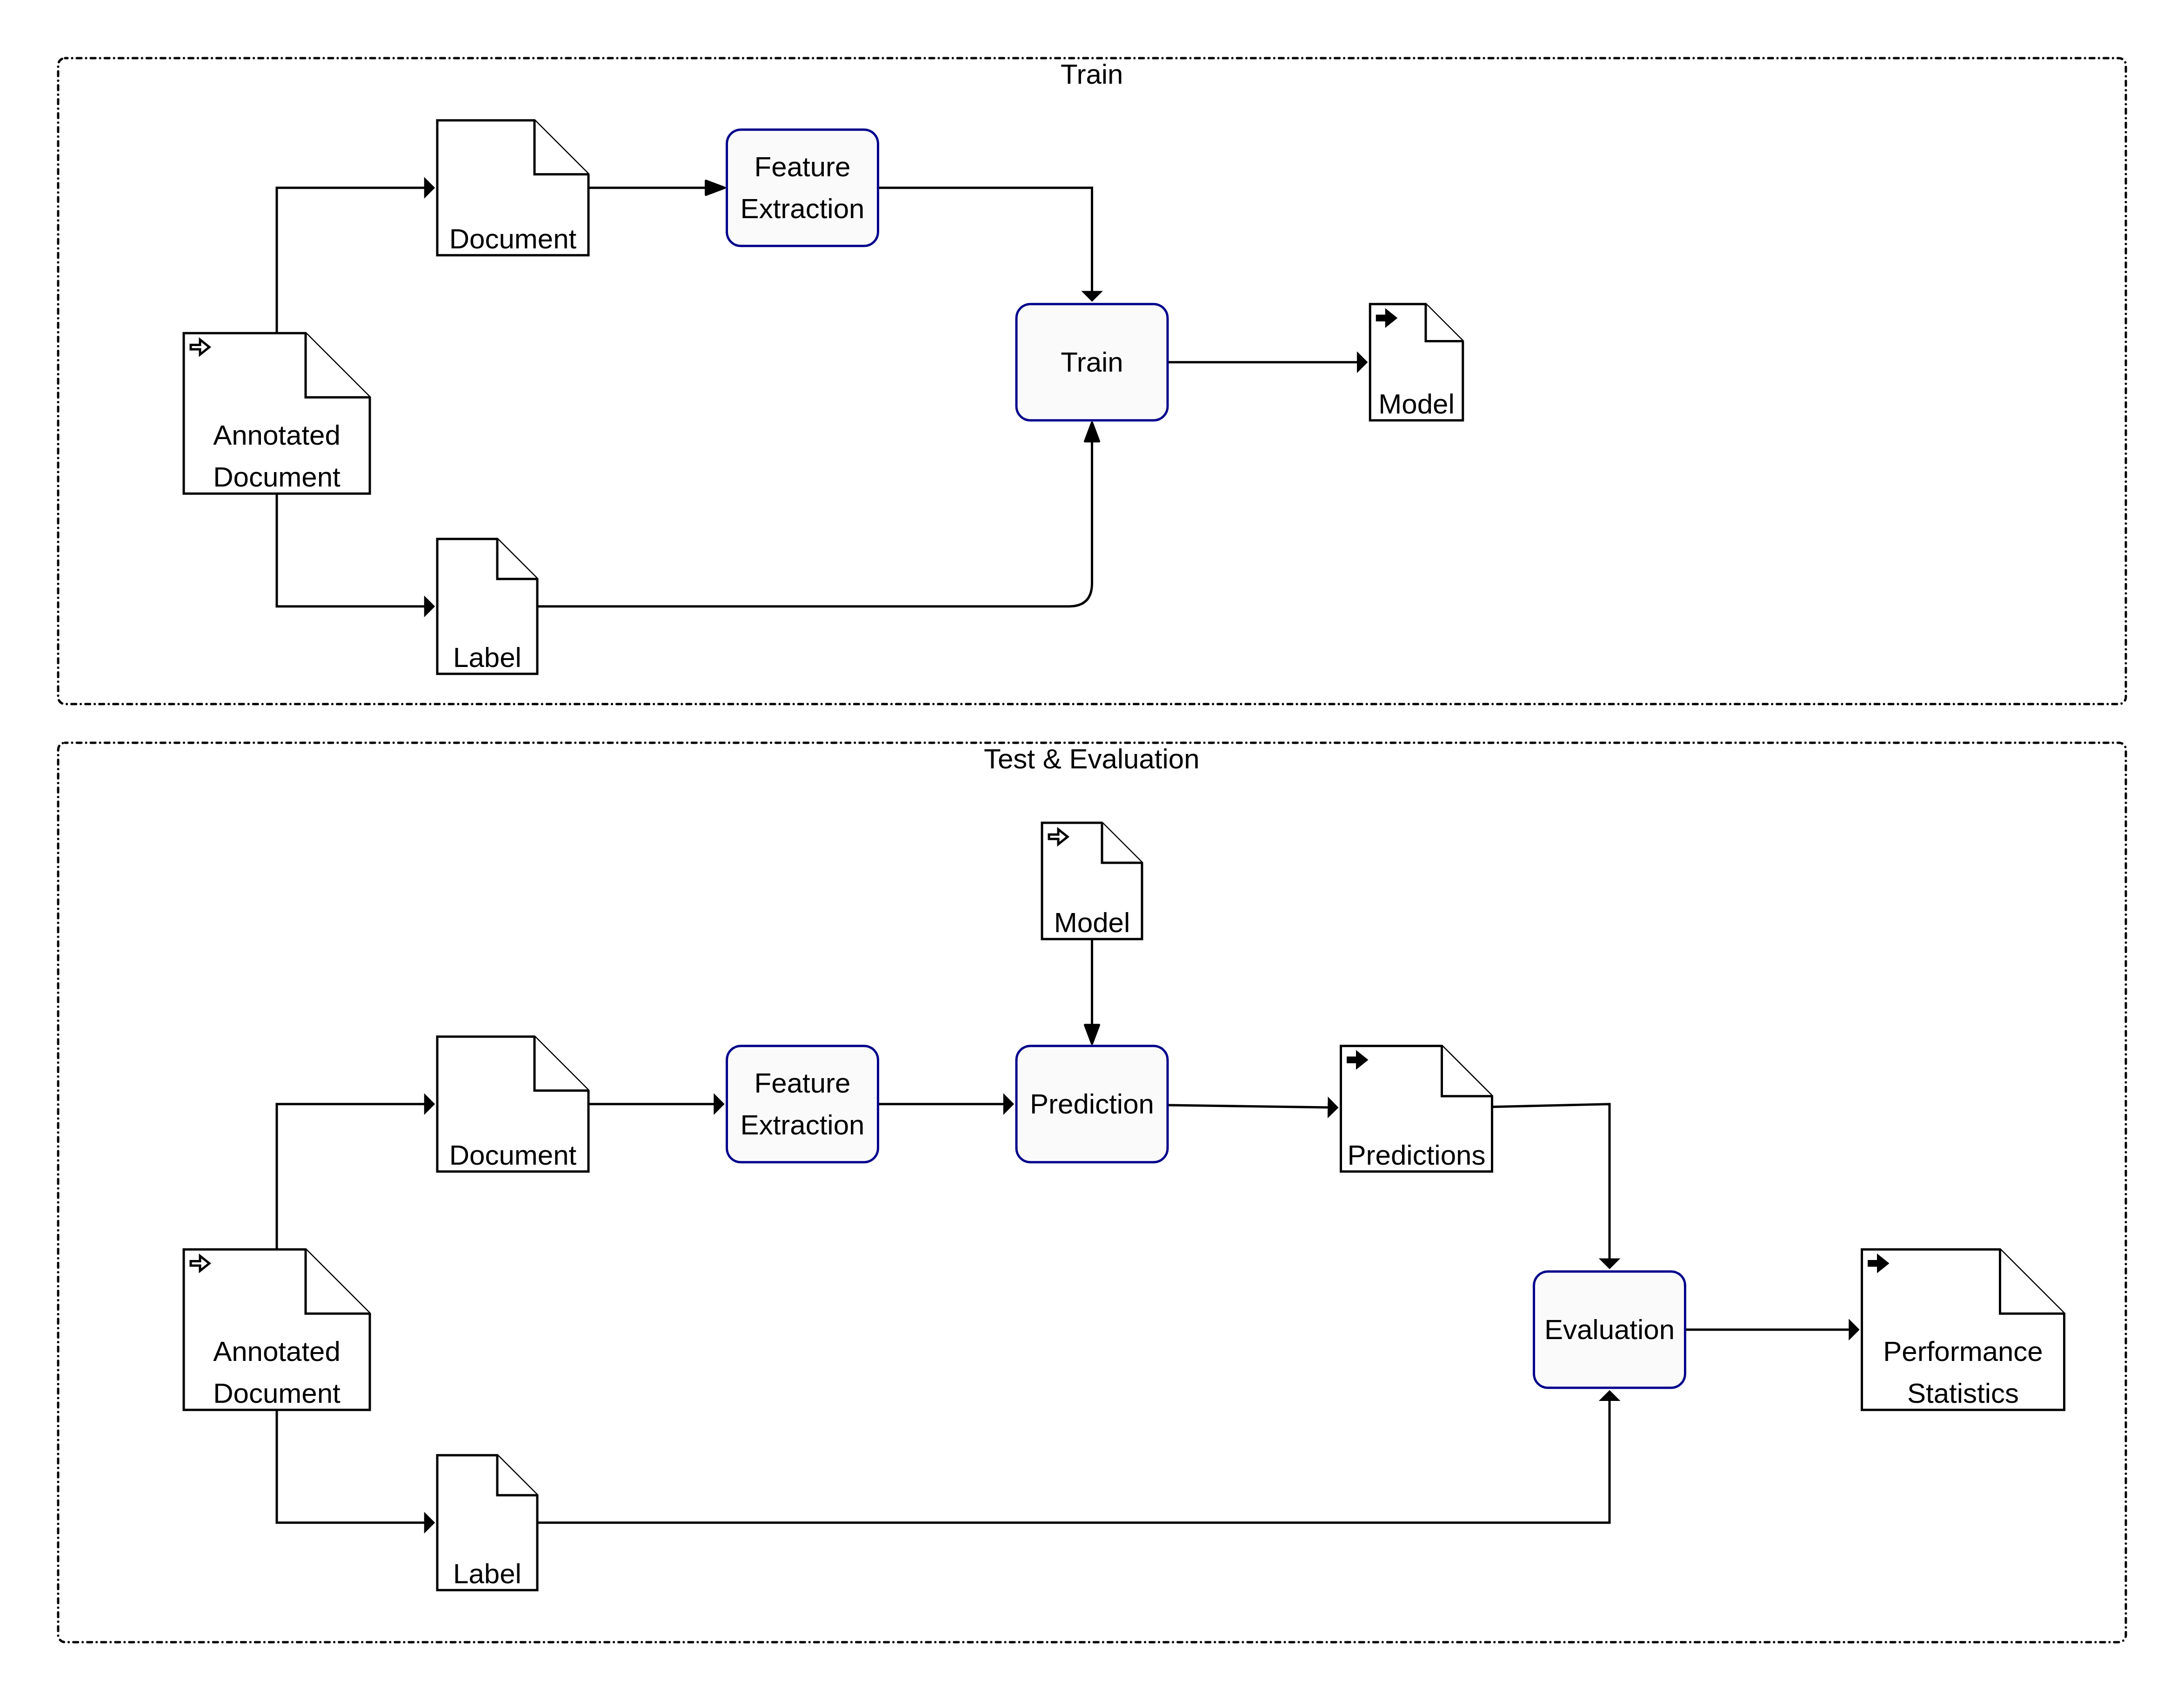
\includegraphics[width=\linewidth]{img/train_and_test.png}
		\end{center}
		\caption{High level overview of training, testing and evaluation of a NER system.}
		\label{fig:overview}
	\end{figure}


	\section{Dataset}
	
	Two very different datasets were used to train and test the NER systems. On the one hand, the famous CoNLL 2003 \cite{tjongkimsang2003conll} dataset, which consists of newswire articles from the Reuters corpus, and on the other hand the W-NUT 2017 \cite{derczynski2017results} dataset, which consists of noisy user-generated text, were used.
	
	The CoNLL 2003 dataset provides an English and a German corpus, but the implemented NER systems were just trained with the English part of the dataset. The English corpus contains almost 1400 news articles, with more than 22.000 sentences in total, from Reuters \cite{reuters}.
	
	In contrast to the CoNLL 2003 dataset, the W-NUT 2017 dataset contains noisy and informal text. Sources of the dataset include posts form social media platforms, online reviews, crowdsourced data, web forums, clinical records and language learner essays. The W-NUT dataset was created as a part of a shared tasked, which aimed to improve NER systems for \textit{emerging} (new named entities, not available in older datasets) and rare (not more than \textit{k} occurrences in the dataset) named entities. The dataset contains 2295 texts from online platforms like Twitter, Reddit, StackExchange and YouTube.
	
	Both datasets are provided via text files. Table \ref{tab:format} shows the format of the CoNLL 2003 dataset. Per word in a sentence, there is one line in the dataset, and one empty line between the sentences. At the end of each line, there is a label, which indicates the type of named entity. 'O' means that the word is no named entity at all, otherwise, the named entity is given in the format 'I-XXX', where XXX stands for the abbreviation of the named entity. If two named entities are next to each other, the second will be tagged in the format 'B-XXX', to make a proper separation possible. The CoNLL dataset provides four different types of named entities: \begin{enumerate*}
		\item persons (PER),
		\item organizations (ORG),
		\item locations (LOC), and
		\item miscellaneous (MISC).
	\end{enumerate*}
	Between the actual word and the label, there are two more columns: the part-of-speech (POS) tag and the words chunk tag. Those two columns provide additional information that is not needed, but they can be used as feature values for machine learning algorithms. 
	
	The W-NUT 2017 dataset comes in a similar format as the CoNLL 2003 dataset, but without the columns for the POS and chunk tag. The W-NUT dataset provides six types of named entities: 
	\begin{enumerate*}
		\item persons,
		\item locations,
		\item corporations,
		\item consumer goods,
		\item creative work, and
		\item groups.
	\end{enumerate*}
In the W-NUT dataset, the separation of named entities is handled differently. Here the first word of a named entity is denoted by 'B-XXX' and subsequent words of the same entity by 'I-XXX'.
	
	\begin{center}
	\begin{table}
		\centering
		\begin{tabular}{l l l l}
			U.N. & NNP & I-NP & I-ORG 
			\\
			official & NN & I-NP & O 
			\\
			Ekeus & NNP & I-NP & I-PER \\ 
			heads & VBZ & I-VP & O 
			\\
			for & IN & I-PP & O \\
			Baghdad & NNP & I-NP & I-LOC \\ 
			. & . & O & O \\
		\end{tabular}
		\caption{Format of the CoNLL dataset.}
		\label{tab:format}
	\end{table}
	\end{center}
	
	
	\section{Implementation}
	
	The following section presents the implementation details of the developed NER systems. Subsection \ref{sub:CRF} starts with presenting the CRF approach. Second, Subsection \ref{sub:lstm} continues with the details of the LSTM approaches.
	
	\subsection{Conditional Random Fields}
	\label{sub:CRF}
	
	The CRF approach was implemented with the help of the following Python libraries: \textit{python-crfsuite} \cite{pycrfsuite}, \textit{Natural Language Toolkit} (NLTK) \cite{nltk}, \textit{scikit-learn} \cite{scikitlearn} and \textit{gensim} \cite{gensim}.
	python-crfsuite is a Python wrapper of CRFsuite \cite{CRFsuite}. The library provides a fast implementation of CRFs, written in C/C++. NLTK is one of the most used Python libraries for natural language processing. It contains many text corpora, text pre-processing functionalities and APIs to other machine learning libraries. NLTK was mainly used because of the included text corpora, that were needed for feature extraction (see Subsection \ref{sec:dic}). scikit-learn is a machine learning Python library that was used for some pre-processing (splitting of train/test data). Last, \textit{gensim}, is a Python library for unsupervised semantic modelling from natural text. It was also used for feature extraction (see the word2vec implementation in Section \ref{sec:unsuperfeat}).
	
	A lot of effort was invested to come up with a good working feature set. The employed feature functions can be grouped into five categories: 
	\begin{enumerate}
		\item word-based features,
		\item sentence \& collection-based features,
		\item dictionary-based features, 
		\item features form other NLP tasks, and
		\item features from unsupervised machine learning algorithms.
	\end{enumerate}

	The five categories listed above are investigated in more detail in the following sub-sections.

	\subsubsection{Word-based features}
	
	Various word-based features were employed in the CRF based NER system. The length of a word was used as a feature value, and if the word starts with an upper-case letter. Additionally, it was checked if the word contains an upper-case letter, a digit or some other special character (like @, -, /). Tkachenko et al. showed an additional word-based feature, the \textit{word-shape} (also called orthographic feature), in \cite{tkachenko2012named}. The shape of a word can be derived by a mapping function. At first each upper-case letter is mapped to an \textit{A}, and every lower-case letter is mapped to an \textit{a}. Digits are all mapped to \textit{9}, and special characters are mapped to \#. Afterwards, subsequent duplicates of the remaining characters are replaced by a + symbol. Examples of some word to word-shape mappings can be seen in Table \ref{tab:wordshape}.
	
	\begin{center}
		\begin{table}[H]
			\centering
			\begin{tabular}{l | l}
				Word & Word-shape \\
				\hline
				Word & Aa+ \\
				WORD & A+ \\
				2020-01-16 & 9999\#99\#99			
			\end{tabular}
			\caption{Examples of word to word-shape mappings.}
			\label{tab:wordshape}
		\end{table}
	\end{center}

	\subsubsection{Sentence \& collection-based features}	
	
	The position of a word in a sentence was used as a sentence-based feature. This may be a helpful feature because the probability of a named entity occurring at the first or last position of a sentence is not the same as on other arbitrary positions.
	
	The overall number of occurrences of the word in the collection was used as a feature because named entities are usually less frequent in datasets than other words (for example stop-words).
	
	\subsubsection{Dictionary-based features}
	\label{sec:dic}
	
	For gathering dictionary features each word was looked up in multiple dictionaries. Four types of dictionaries where used:
	\begin{enumerate*}
		\item stop-words,
		\item name-list,
		\item word-list, and
		\item WordNet \cite{wordnet}.
	\end{enumerate*}

	The stop-word list, the name-list and the word-list are provided by the NLTK library. Stop-words are usually the most common words (such as \textit{is}, \textit{in}, \textit{a}, \textit{that}, etc.) in languages, that give little to no semantics to a sentence. The NLTK stop-word corpus contains 179 words.
	
	The NLTK name-list corpus is a list of almost 8.000 person names, and the word-list is an English dictionary, containing over 230.000 words.
	 
	WordNet is a large lexical database, that contains information like synonyms, antonyms, hyponyms, meronyms, etc. The length of the hypernym path (how many hypernyms or umbrella terms a word has) is used as a feature value. This gives some kind of information like the specificness or rareness of a word.

	\subsubsection{Features from other NLP tasks}
	
	The part-of-speech (POS) tag, which was extracted by the help of the library NLTK, was used as a feature. The process of assigning words into categories is called part-of-speech tagging. A category is formed by words that have similar grammatical properties. Common categories are nouns, verbs, adjectives, etc.
	
	\subsubsection{Features from unsupervised machine learning algorithms}
	\label{sec:unsuperfeat}
	Several features were collected from unsupervised ML clustering algorithms. The cluster which the word appears in is used as a feature value.
	Following algorithms were used: \begin{enumerate*}
		\item Brown clusters, 
		\item Latent-Dirichlet-Allocation, 
		\item and Word2vec.
	\end{enumerate*}

	\textbf{Brown cluster} \cite{brown1992class}. A brown cluster is a hierarchical clustering algorithm that tries to group words of similar semantics. The intuition of the algorithm is that similar words will appear in similar contexts. The output of the algorithm is a dendrogram. The path from the cluster to the root, encoded as a bit sequence, and the cluster itself is used as a feature. The best results were achieved with five clusters. The implementation of the brown clustering algorithm is available on GitHub \cite{brownimp}.
	
	\textbf{Latent Dirichlet Allocation} (LDA) \cite{blei2003latent}. LDA is used to model the abstract topic of a document. It returns the distribution of topics per word. The most dominant topic of each word was used as a feature. The best results were achieved with three topics. LDA topic modelling is contained in the sci-kit learn \cite{scikitlearn} library.
	
	\textbf{Word2Vec cluster}. Word2Vec learns relationships between words and outputs one vector for each word. It maps similar words to similar vectors. The vector is used as a feature. The implemented NER system used the gensim \cite{w2vgensim} implementation of Word2Vec.
	
	\subsection{LSTM Network}
	\label{sub:lstm}
	
	Two variants of LSTM based NER systems were implemented, as they were first proposed by Huang et al. in \cite{huang2015bidirectional}.  Both proposals use a bidirectional LSTM layer, which means that the LSTM network is duplicated. The input as-is is feed into the first layer, the input reversed is feed into the second layer. This can be beneficial because it requires contextual information about past (words to the left of current) and future (words on the right of current) words to correctly classify a named entity.
	
	
	For the implementation of the two variants of LSTM networks the Python deep learning package Keras \cite{keras} was used with TensorFlow \cite{tensorflow} as a back-end. Keras provides a high-level API for creating neural networks, and was designed to conduct experiments fast.
	

	The model of the neural network, which was exported from Keras, of the BI-LSTM approach is shown in Figure \ref{fig:lstm}. After the input layer, strings are converted to vectors in the embedding layer. The embedding layer was pre-trained with GloVe \cite{glove} embeddings with a vector size of 100. After embedding the words, a Dropout layer is applied to avoid over-fitting. The theory behind the Dropout layer was proposed by Srivastava et al. in \cite{srivastava2014dropout}. The key idea is to randomly drop a defined amount of units in training. The dropout rate was set to $0.2$ in the tool. Next, the data flows into the bidirectional LSTM layer. A time distributed dense layer is then applied before output. A time distributed dense layer is used here instead of a normal dense layer because of the sequential nature of natural language: there is one output (named entity label) per time-step or word.

	\begin{figure}
		\begin{center}
			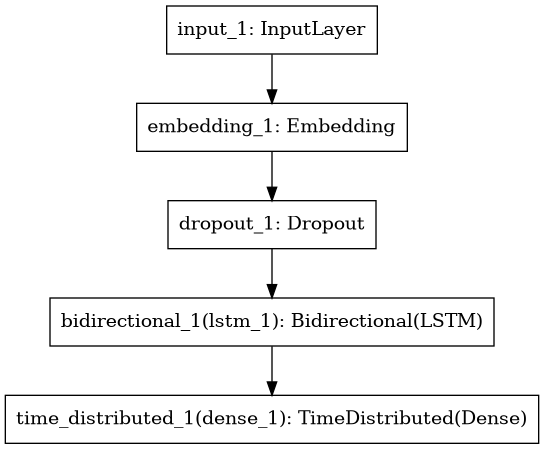
\includegraphics[width=0.5\linewidth]{img/lstm_model.png}
		\end{center}
		\caption{Visualization of the neural network model (exported from Keras) of the NER system with Bidirectional-LSTM network.}
		\label{fig:lstm}
	\end{figure}

	The model of the neural network of the BI-LSTM-CRF approach is shown in Figure \ref{fig:lstm}. It is the same model as described in the previous paragraph, with an additional CRF layer added at the bottom. It is a combination of the first presented CRF approach and the BI-LSTM approach presented before. The CRF layer has the advantage that it does also capture sentence level tag information, instead of just using past and future features as the BI-LSTM approach.
	
	\begin{figure}
		\begin{center}
			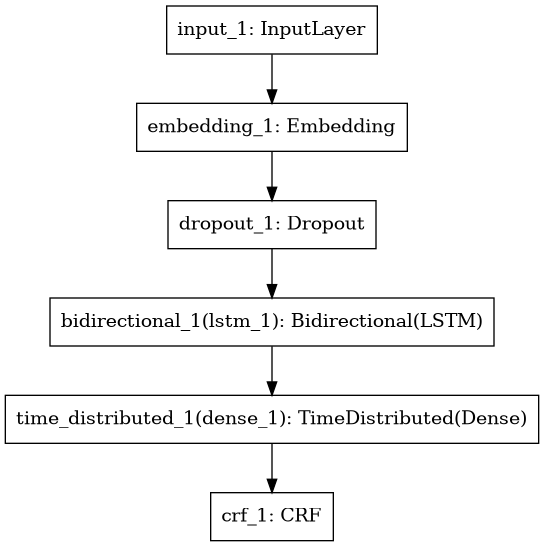
\includegraphics[width=0.5\linewidth]{img/lstm_crf_model.png}
		\end{center}
		\caption{Visualization of the neural network model (exported from Keras) of the NER system with Bidirectional-LSTM-CRF network.}
		\label{fig:lstm-crf}
	\end{figure}
	

	\chapter{Evaluation}
	\label{chap:evaluation}
	
	The evaluation was done, as described in the shared tasked CoNLL 2003 \cite{tjongkimsang2003conll}, by marking predicted named entities as correct \textit{iff} it is an \textit{exact} match with the test data file. For example: if a named entity consists of three words, and one of the three words was mispredicted, the prediction as a whole is considered wrong.
	The CoNLL 2003 shared task provides an evaluation script \cite{conllevalperl}, that was originally written in Perl. The script was later translated to Python and is now available on GitHub, in \cite{conlleval}. This script was used to evaluate the performance of both NER systems on the CoNLL 2003 and the W-NUT 2017 dataset. The evaluation script takes a text file as input, which is produced by the implemented NER systems. The file format is shown in Table \ref{tab:evalformat}. The first column displays the word, the second column the predicted named entity category, and the third column shows the actual named entity category as it was in the original dataset. \\
	
	The remainder of this chapter is structured as follows: Section \ref{sec:results} shows the measured performance of the implemented NER systems. Section \ref{sec:discussion} discusses the results and compares them to related works. Finally, Section \ref{sec:limitations} presents some Limitations of the conducted comparison.
	
	
	\begin{center}
		\begin{table}
			\centering
			\begin{tabular}{l l l}
				U.N. & I-ORG & I-ORG \\
				official & O & O \\
				Ekeus & I-PER & I-PER \\ 
				heads & O & O \\
				for & O & O \\
				Baghdad & I-LOC & I-LOC \\ 
				. & O & O \\
			\end{tabular}
			\caption{Format of file generated by the implemented NER systems.}
			\label{tab:evalformat}
		\end{table}
	\end{center}
		
	\section{Results}
	\label{sec:results}
	
	The measured performance of the implemented NER systems is shown in Table \ref{tab:res_conll} and Table \ref{tab:res_wnut}. Both tables also show the current state-of-the-art performance, that was reached with a tool called \textit{Flair} \cite{akbik2019flair}. Flair also uses a BI-LSTM-CRF model, but it was implemented with the deep learning library PyTorch \cite{pytorch} instead of Keras. What makes their approach different is a new type of string embedding, the so-called Flair embeddings, which are proposed by Akbik et al. in \cite{akbik2018contextual}. The authors published their performance results only based on the F1-score, therefore the precision and recall values of their system are not given in tables.
	
	Table \ref{tab:res_conll} shows precision, recall and F1-score on the CoNLL 2003 dataset. The general observing of this table is that the deep learning approach BI-LSTM-CRF performed better than the machine learning approach CRF on all metrics. Furthermore, the BI-LSTM-CRF approach outperformed the BI-LSTM approach in terms of precision and F1-score. The best implemented variant (BI-LSTM-CRF) is by around 5\% off the results of the state-of-the-art tool Flair.
	
	Table \ref{tab:res_wnut} show precision, recall and F1-score on the W-NUT 2017 dataset. The key finding here is that the CRF and BI-LSTM-CRF approaches performed much better than the non-CRF approach BI-LSTM.
	
	The best performance on the W-NUT 2017 dataset achieved an F1-score of 40.53 \%, while the best result on the CoNLL 2003 dataset was 87.78 \%. The big differences in the performance measurements are a consequence of the two different natures of the datasets. While the CoNLL 2003 dataset consists of very clean, formal texts from newswire articles, the texts used in the W-NUT 2017 dataset are noisy and informal. Furthermore, the texts in the corpus are chosen in a way that the contained named entities are rare (named entities have a low collection frequency). However, this does not imply that the implemented NER systems work better on clean and formal texts, because the difference between the state-of-the-art approaches and the best variant of our approach does not vary a lot (about 3-4\%).
	
	
	\begin{table}
		\begin{center}
			\begin{tabular}{| l | c | c | c |}
				\hline
				Method & Precision & Recall & F1-score \\ \hline
				CRF & 84.25 & 85.42 & 84.83 \\ \hline
				BI-LSTM & 84.37 & \textbf{86.58} & 85.46 \\ \hline
				BI-LSTM-CRF & \textbf{89.41} & 86.20 & \textbf{87.78} \\ \hline
				Flair & - & - & 93.09 \\ \hline
			\end{tabular}
		\end{center}
		\caption{Results on CoNLL 2003 dataset.}
		\label{tab:res_conll}
	\end{table}

	\begin{table}
		\begin{center}
			\begin{tabular}{| l | c | c | c |}
				\hline
				Method & Precision & Recall & F1-score \\ \hline
				CRF & 31.54 & \textbf{56.72} & \textbf{40.53} \\ \hline
				BI-LSTM & 8.69 & 23.16 & 12.63 \\ \hline
				BI-LSTM-CRF & \textbf{33.61} & 31.03 & 32.27 \\ \hline
				Flair & - & - & 49.49 \\ \hline
			\end{tabular}
		\end{center}
		\caption{Results on W-NUT 17 dataset.}
		\label{tab:res_wnut}
	\end{table}

	\section{Discussion}
	\label{sec:discussion}

	The observations that were made by Ljube{\v{s}}i{\'c} in \cite{ljubevsic2018comparing} could be reproduced only partially. The authors claimed, that in general the BI-LSTM variant performed better than the CRF approach, but with an optimal feature set, CRFs came close to the results of BI-LSTM approach. Furthermore, Ljube{\v{s}}i{\'c} states that the difference between the approaches increases with non-standardness of the dataset (in favour of the BI-LSTM approach). The first claim conforms with the data shown in Table \ref{tab:res_conll} because the BI-LSTM approach performed a little bit better than the CRF approach. However, the second claim could not be confirmed. The texts in the W-NUT 2017 dataset are containing less \textit{standard} named entities than the texts in the CoNLL 2003 dataset. According to Ljube{\v{s}}i{\'c}, the BI-LSTM approach should perform better than the CRF approach on the W-NUT 2017 dataset (in comparison to the results achieved for the CoNLL 2003 dataset), which is not true in our case. In our case, the CRF approach performed much better, in comparison to the BI-LSTM approach, on W-NUT 2003 dataset than it did on the CoNLL dataset.
	
	The CRF approach reached an F1 score of 84.83\% on the CoNLL 2003 dataset. This shows that the CRF approach presented by McCallum et al. in \cite{mccallum2003early}, which participated in the CoNLL 2003 shared task, could be reproduced. In  \cite{tjongkimsang2003conll}, the reported F1-score of their system is 84.04\%.
	
	The results in Table \ref{tab:res_wnut} conform to the comparison published by Derczynski et al. in \cite{derczynski2017results}. The three systems achieving the highest scores are all using CRF classifiers (in combination with other techniques). In our case, the methods using a CRF classifier also performed much better than the BI-LSTM approach.
	
	\section{Limitations}
	\label{sec:limitations}
	
	One limitation of the comparison is that the implemented approaches were trained with a different train/test split. Teams that participated in the CoNLL 2003 shared task used a fixed train/test split of approximately $75\% / 25\%$, and they used about $23\%$ of the data as a development set for fine-tune. The implemented NER systems used a train/test split of $85\% / 15\%$ that was chosen randomly, and no a development set was used. The results are therefore not completely comparable with other participants of the CoNLL and W-NUT competition.
	
	Second, the limits of the variations of the F1-score, as it was done in the CoNLL 2003 shared task, should be calculated and specified in Table \ref{tab:res_conll} and Table \ref{tab:res_wnut}.

	\chapter{Conclusion}
	\label{chap:conclusion}
	
	Aim of this thesis was to perform a practical study, comparing two different approaches of NER systems regarding their performance on different datasets. 
	The first system (CRF system), the traditional machine learning approach, was implemented by the use of Conditional Random Fields, while the second system (LSTM system), a modern deep learning approach, was implemented with a Long-Short-Term-Memory neural network. The LSTM system comes in two variants: a bidirectional LSTM (BI-LSTM) network, and a BI-LSTM-CRF network, which is a combination of the CRF and the BI-LSTM system. The implemented NER systems were compared by there performance of two different datasets, the CoNLL 2003 and the W-NUT 2017 dataset.
	
	In Chapter \ref{chap:evaluation} it was shown, that the LSTM approach performed better on the CoNLL 2003 dataset. However, the CRF approach performed very well on the noisy W-NUT 2017 dataset. The BI-LSTM-CRF is the current state-of-the-art model to many NLP tasks, including NER. Nevertheless, the additional use of CRFs can boost the performance of LSTM based approaches. They are used in many state-of-the-art tools, especially those focusing on noisy texts, in combination with deep learning algorithms.
	
	Both NER systems still have some potential for improvement. Future work could be:
	\begin{enumerate*}
		\item use a feature selection algorithm (univariant selection or recursive feature elimination) for fine-tuning the CRF system,
		\item replace the GloVe string embeddings by more recent embedding techniques, like BERT \cite{devlin2018bert}, ELMo \cite{peters2018deep}, or Flair \cite{akbik2018contextual} embeddings.
	\end{enumerate*}

	To provide a more comprehensive comparison, it would also be necessary to measure the performance on additional datasets or include non-English data. Another goal could be to add more implementation variants to the comparison. Finally, an error analysis, which elaborates in which cases CRFs perform better then LSTM networks and vice versa, could give hints on how NER systems can be improved further.
	
	\bibliographystyle{plain}
	\bibliography{thesis}

\end{document}
